\documentclass[12pt,]{article}
\usepackage{lmodern}
\usepackage{setspace}
\setstretch{1.5}
\usepackage{amssymb,amsmath}
\usepackage{ifxetex,ifluatex}
\usepackage{fixltx2e} % provides \textsubscript
\ifnum 0\ifxetex 1\fi\ifluatex 1\fi=0 % if pdftex
  \usepackage[T1]{fontenc}
  \usepackage[utf8]{inputenc}
\else % if luatex or xelatex
  \ifxetex
    \usepackage{mathspec}
  \else
    \usepackage{fontspec}
  \fi
  \defaultfontfeatures{Ligatures=TeX,Scale=MatchLowercase}
    \setmainfont[]{NanumGothic}
\fi
% use upquote if available, for straight quotes in verbatim environments
\IfFileExists{upquote.sty}{\usepackage{upquote}}{}
% use microtype if available
\IfFileExists{microtype.sty}{%
\usepackage{microtype}
\UseMicrotypeSet[protrusion]{basicmath} % disable protrusion for tt fonts
}{}
\usepackage[margin=1in]{geometry}
\usepackage{hyperref}
\hypersetup{unicode=true,
            pdftitle={CLI vs GUI 내전},
            pdfauthor={이정훈, CLI 종족 지도자},
            pdfborder={0 0 0},
            breaklinks=true}
\urlstyle{same}  % don't use monospace font for urls
\usepackage{longtable,booktabs}
\usepackage{graphicx,grffile}
\makeatletter
\def\maxwidth{\ifdim\Gin@nat@width>\linewidth\linewidth\else\Gin@nat@width\fi}
\def\maxheight{\ifdim\Gin@nat@height>\textheight\textheight\else\Gin@nat@height\fi}
\makeatother
% Scale images if necessary, so that they will not overflow the page
% margins by default, and it is still possible to overwrite the defaults
% using explicit options in \includegraphics[width, height, ...]{}
\setkeys{Gin}{width=\maxwidth,height=\maxheight,keepaspectratio}
\IfFileExists{parskip.sty}{%
\usepackage{parskip}
}{% else
\setlength{\parindent}{0pt}
\setlength{\parskip}{6pt plus 2pt minus 1pt}
}
\setlength{\emergencystretch}{3em}  % prevent overfull lines
\providecommand{\tightlist}{%
  \setlength{\itemsep}{0pt}\setlength{\parskip}{0pt}}
\setcounter{secnumdepth}{5}
% Redefines (sub)paragraphs to behave more like sections
\ifx\paragraph\undefined\else
\let\oldparagraph\paragraph
\renewcommand{\paragraph}[1]{\oldparagraph{#1}\mbox{}}
\fi
\ifx\subparagraph\undefined\else
\let\oldsubparagraph\subparagraph
\renewcommand{\subparagraph}[1]{\oldsubparagraph{#1}\mbox{}}
\fi

%%% Use protect on footnotes to avoid problems with footnotes in titles
\let\rmarkdownfootnote\footnote%
\def\footnote{\protect\rmarkdownfootnote}

%%% Change title format to be more compact
\usepackage{titling}

% Create subtitle command for use in maketitle
\newcommand{\subtitle}[1]{
  \posttitle{
    \begin{center}\large#1\end{center}
    }
}

\setlength{\droptitle}{-2em}

  \title{CLI vs GUI 내전}
    \pretitle{\vspace{\droptitle}\centering\huge}
  \posttitle{\par}
    \author{이정훈, CLI 종족 지도자}
    \preauthor{\centering\large\emph}
  \postauthor{\par}
      \predate{\centering\large\emph}
  \postdate{\par}
    \date{2018년 12월}

% rstudio/bookdown preamble.tex
% https://github.com/rstudio/bookdown/blob/master/inst/examples/latex/preamble.tex

\usepackage{booktabs}
\usepackage{longtable}
\usepackage[bf,singlelinecheck=off]{caption}

% \setmainfont[UprightFeatures={SmallCapsFont=AlegreyaSC-Regular}]{Alegreya}

\usepackage{framed,color}
\definecolor{shadecolor}{RGB}{248,248,248}

\renewcommand{\textfraction}{0.05}
\renewcommand{\topfraction}{0.8}
\renewcommand{\bottomfraction}{0.8}
\renewcommand{\floatpagefraction}{0.75}

\renewenvironment{quote}{\begin{VF}}{\end{VF}}
\let\oldhref\href
\renewcommand{\href}[2]{#2\footnote{\url{#1}}}

\ifxetex
  \usepackage{letltxmacro}
  \setlength{\XeTeXLinkMargin}{1pt}
  \LetLtxMacro\SavedIncludeGraphics\includegraphics
  \def\includegraphics#1#{% #1 catches optional stuff (star/opt. arg.)
    \IncludeGraphicsAux{#1}%
  }%
  \newcommand*{\IncludeGraphicsAux}[2]{%
    \XeTeXLinkBox{%
      \SavedIncludeGraphics#1{#2}%
    }%
  }%
\fi

\makeatletter
\newenvironment{kframe}{%
\medskip{}
\setlength{\fboxsep}{.8em}
 \def\at@end@of@kframe{}%
 \ifinner\ifhmode%
  \def\at@end@of@kframe{\end{minipage}}%
  \begin{minipage}{\columnwidth}%
 \fi\fi%
 \def\FrameCommand##1{\hskip\@totalleftmargin \hskip-\fboxsep
 \colorbox{shadecolor}{##1}\hskip-\fboxsep
     % There is no \\@totalrightmargin, so:
     \hskip-\linewidth \hskip-\@totalleftmargin \hskip\columnwidth}%
 \MakeFramed {\advance\hsize-\width
   \@totalleftmargin\z@ \linewidth\hsize
   \@setminipage}}%
 {\par\unskip\endMakeFramed%
 \at@end@of@kframe}
\makeatother

\makeatletter
\@ifundefined{Shaded}{
}{\renewenvironment{Shaded}{\begin{kframe}}{\end{kframe}}}
\makeatother

\newenvironment{rmdblock}[1]
  {
  \begin{itemize}
  \renewcommand{\labelitemi}{
    \raisebox{-.7\height}[0pt][0pt]{
      {\setkeys{Gin}{width=3em,keepaspectratio}\includegraphics{images/#1}}
    }
  }
  \setlength{\fboxsep}{1em}
  \begin{kframe}
  \item
  }
  {
  \end{kframe}
  \end{itemize}
  }
\newenvironment{rmdnote}
  {\begin{rmdblock}{note}}
  {\end{rmdblock}}
\newenvironment{rmdcaution}
  {\begin{rmdblock}{caution}}
  {\end{rmdblock}}
\newenvironment{rmdimportant}
  {\begin{rmdblock}{important}}
  {\end{rmdblock}}
\newenvironment{rmdtip}
  {\begin{rmdblock}{tip}}
  {\end{rmdblock}}
\newenvironment{rmdwarning}
  {\begin{rmdblock}{warning}}
  {\end{rmdblock}}

\usepackage{makeidx}
\makeindex

\urlstyle{tt}

\usepackage{amsthm}
\makeatletter
\def\thm@space@setup{%
  \thm@preskip=8pt plus 2pt minus 4pt
  \thm@postskip=\thm@preskip
}
\makeatother

% flush left while keep identation
\makeatletter
\newcommand\iraggedright{%
  \let\\\@centercr\@rightskip\@flushglue \rightskip\@rightskip
  \leftskip\z@skip}
\makeatother

% \frontmatter

\usepackage{amsthm}
\newtheorem{theorem}{Theorem}[section]
\newtheorem{lemma}{Lemma}[section]
\theoremstyle{definition}
\newtheorem{definition}{Definition}[section]
\newtheorem{corollary}{Corollary}[section]
\newtheorem{proposition}{Proposition}[section]
\theoremstyle{definition}
\newtheorem{example}{Example}[section]
\theoremstyle{definition}
\newtheorem{exercise}{Exercise}[section]
\theoremstyle{remark}
\newtheorem*{remark}{Remark}
\newtheorem*{solution}{Solution}
\begin{document}
\maketitle

% align only at left, not at right.
\iraggedright

\section{초록}

GUI 종족과 CLI 종족간의 전쟁은 끝이 보이지 않고 있다. 두 종족간의 전쟁은
윈도우의 출현으로 GUI 종족의 일방적인 승리로 끝날 것으로 보였지만,
클라우드 시대의 출현으로 다시 CLI 종족이 주도권을 잡아가고 있는 모양이
되었다. CLI 종족은 과거 소수였지만, 소프트웨어 카펜트리{[}Simperler and
Wilson
\protect\hyperlink{ref-DBLP:journalsux2fcorrux2fSimperlerW15}{2015}{]}를
내세워서 GUI 종족을 흡수하면서 세력을 급격히 확장시키고 있다.

두 종족간의 전쟁은 어떻게 전개될까? 과연 과학 컴퓨팅{[}Wilson
\protect\hyperlink{ref-10.1371ux2fjournal.pbio.1001745}{2014}{]}는
도움이 될까?

\hypertarget{-}{%
\subsection{종족전쟁 도해}\label{-}}

\begin{figure} [!htb]
\centerline{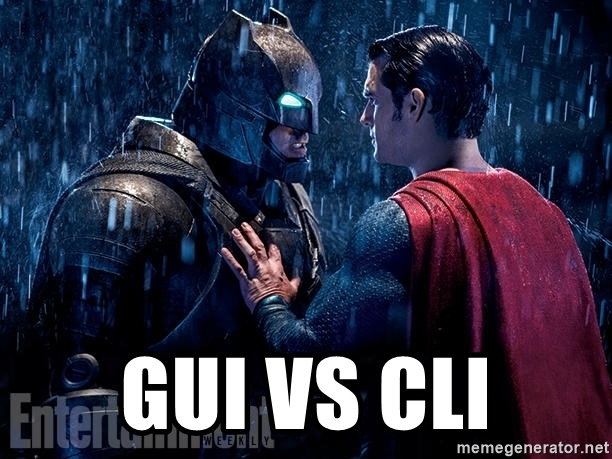
\includegraphics[width=0.2\textwidth]{fig/gui-vs-cli.jpg}}
\caption{GUI vs. CLI}
\end{figure}

\subsection{수식}

\[\text{생산성} = \frac{\text{CLI}^2}{\text{GUI}}\]

\subsection{문제해결}

GUI로 해결하기 힘든 아래와 같이 \texttt{pdf} 파일 생성시 생긴 문제는
구글 검색을 통해서 stackoverflow
\href{https://stackoverflow.com/questions/18178084/pandoc-and-foreign-characters}{Pandoc
and foreign characters}에서 해법을 찾아
\texttt{-\/-latex-engine=xelatex\ -V\ CJKmainfont=NanumGothic}와 같이
글꼴까지 반영시킨다.

\begin{verbatim}
! Package inputenc Error: Unicode character 내 (U+B0B4)
(inputenc)                not set up for use with LaTeX.
\end{verbatim}

\hypertarget{r-}{%
\section{R 코드}\label{r-}}

\subsection{기술통계량}

\begin{verbatim}
##       mpg             cyl             disp             hp       
##  Min.   :10.40   Min.   :4.000   Min.   : 71.1   Min.   : 52.0  
##  1st Qu.:15.43   1st Qu.:4.000   1st Qu.:120.8   1st Qu.: 96.5  
##  Median :19.20   Median :6.000   Median :196.3   Median :123.0  
##  Mean   :20.09   Mean   :6.188   Mean   :230.7   Mean   :146.7  
##  3rd Qu.:22.80   3rd Qu.:8.000   3rd Qu.:326.0   3rd Qu.:180.0  
##  Max.   :33.90   Max.   :8.000   Max.   :472.0   Max.   :335.0  
##       drat      
##  Min.   :2.760  
##  1st Qu.:3.080  
##  Median :3.695  
##  Mean   :3.597  
##  3rd Qu.:3.920  
##  Max.   :4.930
\end{verbatim}

\subsection{회귀모형}

\begin{verbatim}
## # A tibble: 2 x 5
##   term        estimate std.error statistic  p.value
##   <chr>          <dbl>     <dbl>     <dbl>    <dbl>
## 1 (Intercept)  29.6      1.23        24.1  3.58e-21
## 2 disp         -0.0412   0.00471     -8.75 9.38e-10
\end{verbatim}

\subsection{시각화}

\includegraphics{data_science_files/figure-latex/sample-viz-1.pdf}

\hypertarget{-pandoc--}{%
\subsection{\texorpdfstring{첨부: \texttt{pandoc} 컴파일
코드}{첨부: pandoc 컴파일 코드}}\label{-pandoc--}}

\section*{참고문헌}
\addcontentsline{toc}{section}{참고문헌}

\hypertarget{refs}{}
\leavevmode\hypertarget{ref-DBLP:journalsux2fcorrux2fSimperlerW15}{}%
\textsc{Simperler, A. and Wilson, G.} 2015. Software carpentry get more
done in less time. \emph{CoRR} \emph{abs/1506.02575}.

\leavevmode\hypertarget{ref-10.1371ux2fjournal.pbio.1001745}{}%
\textsc{Wilson, D.A.A.B., Greg AND Aruliah}. 2014. Best practices for
scientific computing. \emph{PLOS Biology} \emph{12}, 1, 1--7.


\end{document}
